\section{Calcolo delle metriche}
\subsubsection{Premessa relativa al periodo di progettazione e codifica della Technology Baseline}
Data la natura fortemente mutevole del Proof of Concept è stato deciso di non tenere traccia delle metriche di prodotto durante il suo sviluppo. Infatti, nella fase di progettazione di dettaglio e codifica il prodotto cambierà radicalmente, e non ci sarà una vera e propria continuità rispetto al PoC. \newline
Alcune delle metriche sulla pianificazione non erano calcolabili, in quanto non si può dire di aver effettivamente soddisfatto dei requisiti, dunque si è rinunciato ad utliizzarle.
Cionondimeno, poiché è necessario poter avere una visione dell'andamento del progetto nel tempo, si è deciso di tenere traccia di tutte le metriche a partire dalla fase di progettazione in dettaglio e codifica. Saranno considerate le serie storiche con una quantità maggiore di dati a disposizione.

\subsection{Legenda}
Legenda:
\begin{itemize}
	\item \textbf{-}: campi vuoti;
	\item \textbf{N}: nome del documento;
	\item \textbf{RR}: periodo di revisione dei requisiti;
	\item \textbf{C}: periodo di consolidamento dei requisiti;
	\item \textbf{TB}: periodo di progettazione e codifica della Technology Baseline;
	\item \textbf{PD}: periodo di progettazione di dettaglio e codifica;
	\item \textbf{VC}: periodo di validazione e collaudo.
\end{itemize}


\subsection{EAC - Estimated At Completion}
\begin{longtable}
	{ >{\centering}p{0.15\textwidth}
			>{\centering}p{0.15\textwidth} >{\centering}p{0.15\textwidth} >{\centering}p{0.15\textwidth} >{\centering}p{0.15\textwidth}}
		%\hline
		\rowcolor{white}\caption{EAC nei periodi da RR a TB}\\
		\rowcolorhead
		\textbf{\color{white}RR} 
		& \textbf{\color{white}C} 
		& \textbf{\color{white}TB}
		& \textbf{\color{white}PD}
		& \textbf{\color{white}VC}
		\tabularnewline %\hline  
		\endhead
			
	-
	& \EUR{820,00}
	& \EUR{4245,00}
	& -
	& -
	\tabularnewline %\hline 
\end{longtable}
\begin{figure}[H]
	\centering
	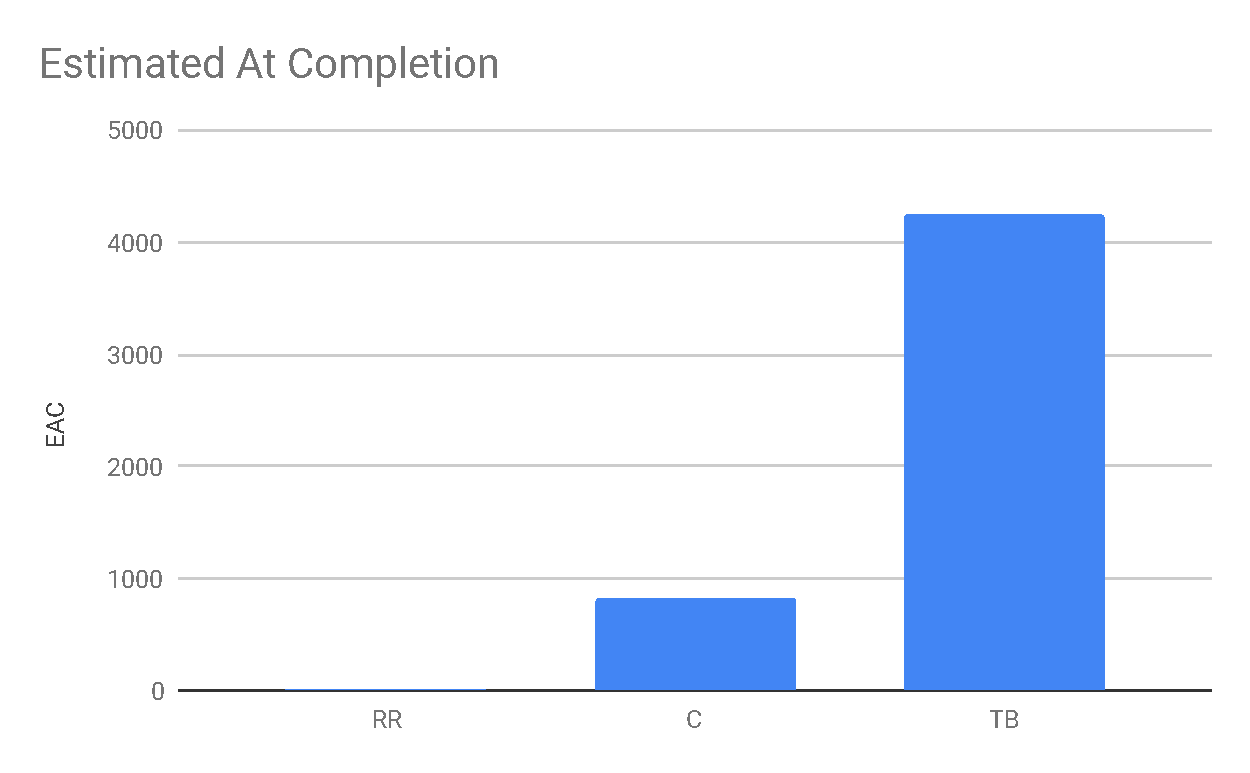
\includegraphics[scale=0.5]{res/images/eac.pdf}
	\caption{Estimated At Completion durante i periodi da RR a TB}
\end{figure}

\subsection{VAC - Variance At Completion}
\begin{longtable}{ >{\centering}p{0.15\textwidth}
		>{\centering}p{0.15\textwidth} >{\centering}p{0.15\textwidth} >{\centering}p{0.15\textwidth} >{\centering}p{0.15\textwidth}}
	%\hline
	\rowcolor{white}\caption{VAC nei periodi da RR a TB}\\
	\rowcolorhead
	\textbf{\color{white}RR} 
	& \textbf{\color{white}C} 
	& \textbf{\color{white}TB}
	& \textbf{\color{white}PD}
	& \textbf{\color{white}VC}
	\tabularnewline %\hline
	\endhead 	
	-
	& 0\%
	& 1.44\%
	& -
	& -
	\tabularnewline %\hline 
	
\end{longtable}
\begin{figure}[H]
	\centering
	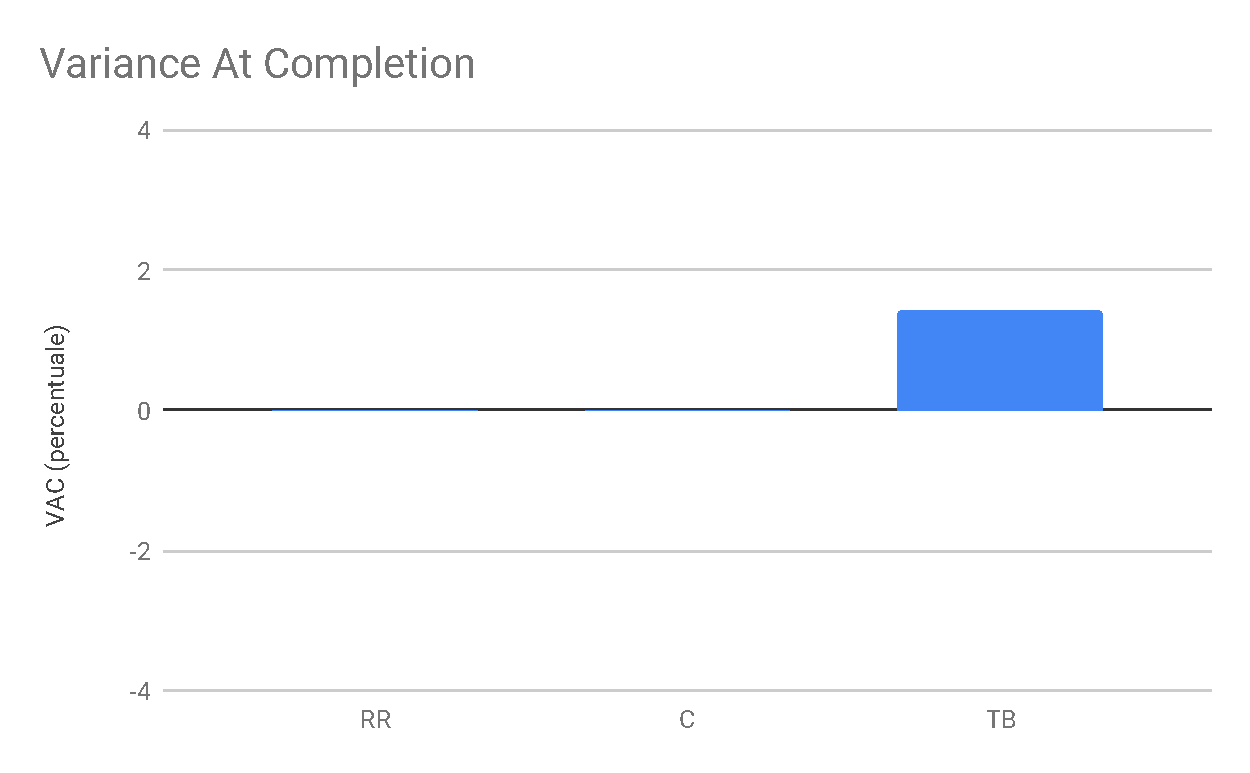
\includegraphics[scale=0.5]{res/images/vac.pdf}
	\caption{Variance At Completion}
\end{figure}
\pagebreak
\subsection{AC - Actual Cost}
\begin{longtable}{ >{\centering}p{0.15\textwidth}
		 >{\centering}p{0.15\textwidth} >{\centering}p{0.15\textwidth} >{\centering}p{0.15\textwidth} >{\centering}p{0.15\textwidth}}
	%\hline
	\rowcolor{white}\caption{AC nei periodi da RR a TB}\\
	\rowcolorhead
	\textbf{\color{white}RR} 
	& \textbf{\color{white}C} 
	& \textbf{\color{white}TB}
	& \textbf{\color{white}PD}
	& \textbf{\color{white}VC}
	\tabularnewline %\hline 	
	-
	& \EUR{820,00}
	& \EUR{4245,00}
	& -
	& -
	\tabularnewline %\hline 	
\end{longtable}
\begin{figure}[H]
	\centering
	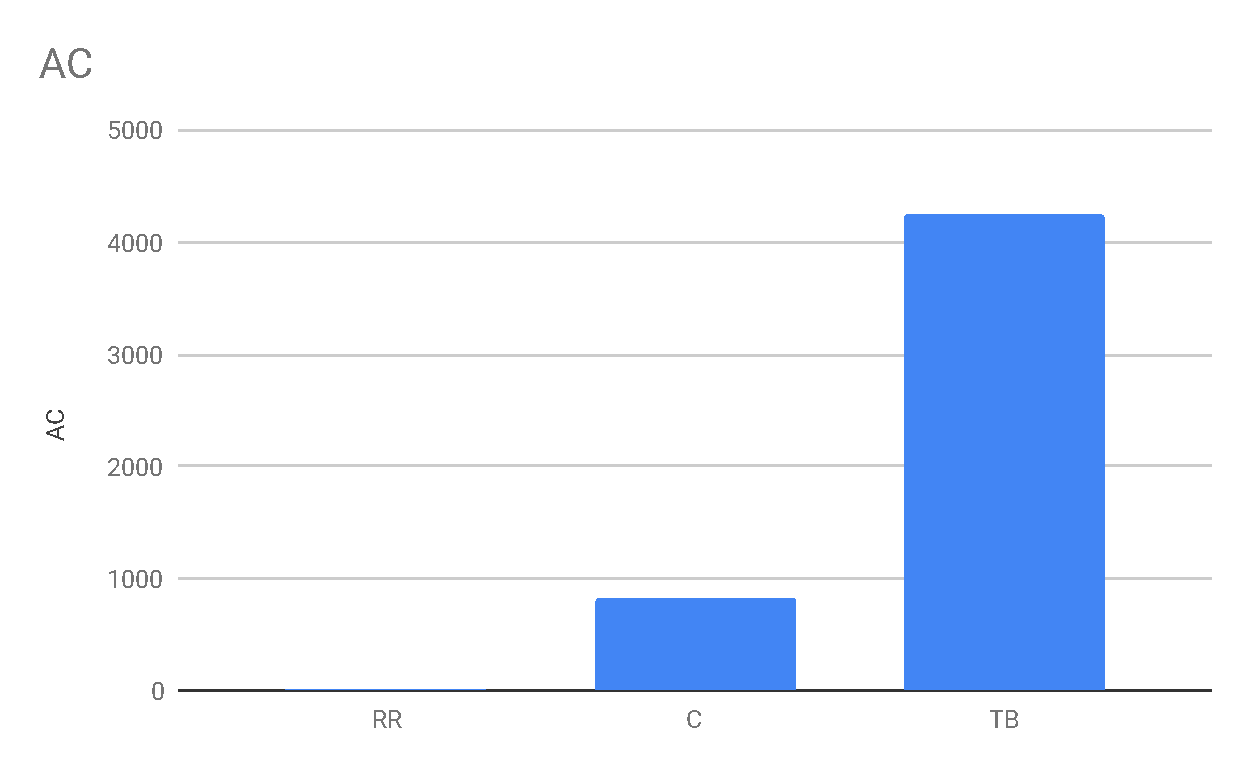
\includegraphics[scale=0.5]{res/images/ac.pdf}
	\caption{Actual Cost}
\end{figure}


\pagebreak
\subsection{Indice di Gulpease}

\begin{longtable}{ >{\centering}p{0.15\textwidth} >{\centering}p{0.10\textwidth}	>{\centering}p{0.1075\textwidth} >{\centering}p{0.10\textwidth} >{\centering}p{0.10\textwidth} >{\centering}p{0.10\textwidth}}
	
	%\hline
	\rowcolor{white}\caption{Indice di Gulpease raggruppato per documento, lungo i periodi da RR a TB}\\
	\rowcolorhead
	\textbf{\color{white}N} 
	& \textbf{\color{white}RR} 
	& \centering\textbf{\color{white}C}
	& \textbf{\color{white}TB}
	& \textbf{\color{white}PD}
	& \textbf{\color{white}VC} 
	\tabularnewline %\hline 	
	
	\textit{Analisi dei requisiti}
	& 67
	& 66
	& 63
	& -
	& -
	\tabularnewline %\hline 
	
	\textit{Glossario}
	& 71
	& 71
	& 71
	& -
	& -
	\tabularnewline %\hline 
	
	\textit{Norme di progetto}
	& 65
	& 65
	& 63
	& -
	& -
	\tabularnewline %\hline 
	
	\textit{Piano di progetto}
	& 68
	& 68
	& 66
	& -
	& -
	\tabularnewline %\hline 
	
	\textit{Piano di qualifica}
	& 70
	& 70
	& 67
	& -
	& -
	\tabularnewline %\hline 
	
	\textit{Studio di Fattibilità}
	& 73
	& -
	& -
	& -
	& -
	\tabularnewline %\hline 
	
	\textit{Verbali esterni (media)}
	& 72
	& 72
	& 66
	& -
	& -
	\tabularnewline %\hline 
	
	\textit{Verbali interni (media)}
	& 74
	& 74
	& 70
	& -
	& -
\end{longtable}
\begin{figure}[H]
	\centering
	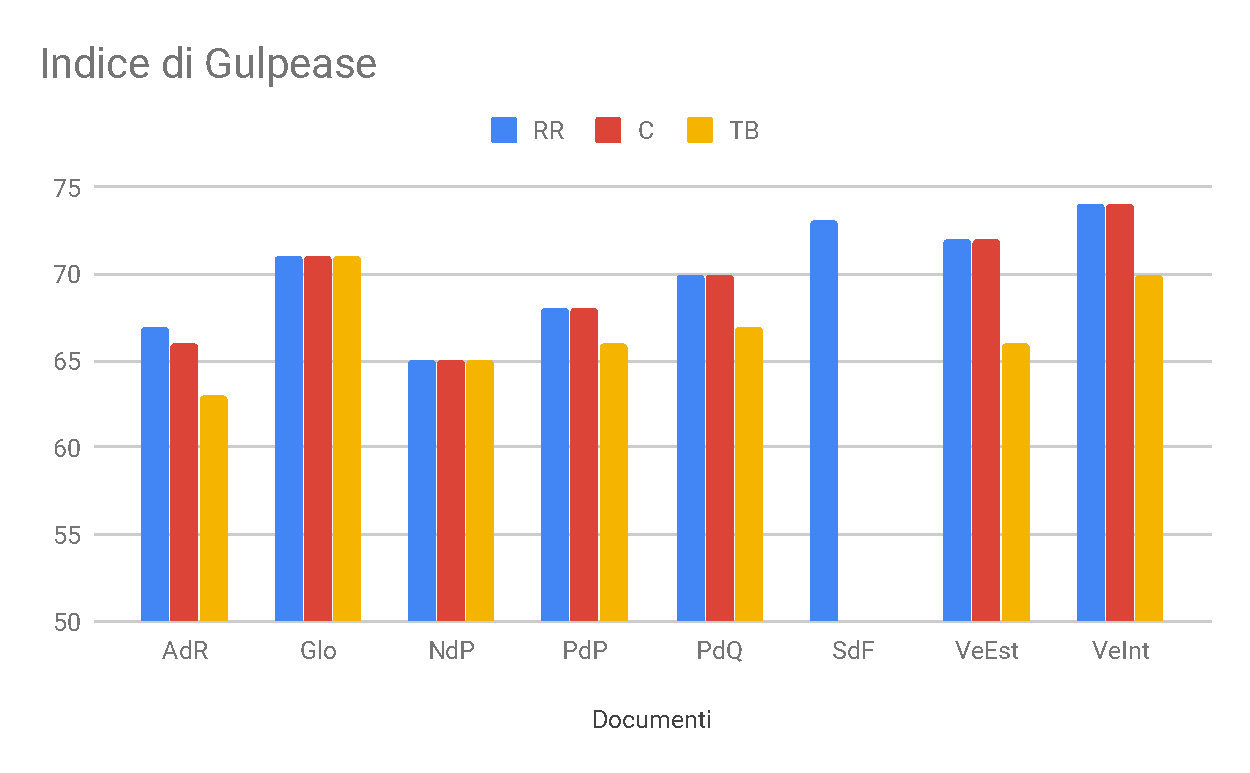
\includegraphics[scale=0.5]{res/images/gulpease.pdf}
	\caption{Indice di Gulpease}
\end{figure}


% questa metrica è stata abolita per volonta di Giacomo Greggio, il Master delle Norme. Sia fatta la sua volontà! Così nel PdQ come nelle Norme.
\begin{comment}
\subsection{PMS - Percentuale di metriche soddisfatte}

\begin{longtable}{ >{\centering}p{0.25\textwidth} >{\centering}p{0.25\textwidth}}
	%\hline
	\rowcolorhead
	\textbf{\color{white}Metrica} 
	& \textbf{\color{white}Soddisfatta?} 
	\tabularnewline %\hline 
		
	EAC
	& sì
	\tabularnewline %\hline
	VAC
	& sì
	\tabularnewline %\hline
	AC
	& sì
	\tabularnewline %\hline
	Gulpease
	& sì
	\tabularnewline %\hline
	\textbf{PMS}
	& \textbf{100\%}
	\tabularnewline %\hline
\end{longtable}
\end{comment}